% Build with: latexmk leanSPHINCS.tex (output in .build/)
\documentclass[11pt]{article}

\usepackage[T1]{fontenc}
\usepackage{lmodern}
\usepackage[margin=1in]{geometry}
\usepackage{microtype}
\usepackage{amsmath,amssymb}
\usepackage{booktabs}
\usepackage{enumitem}
\usepackage{xcolor}
\usepackage[colorlinks=true,linkcolor=blue!50!black,citecolor=blue!50!black,urlcolor=blue!50!black]{hyperref}
\usepackage{cleveref}
\usepackage{tikz}
\usetikzlibrary{calc,decorations.pathreplacing}
\definecolor{newfts}{RGB}{20,70,170}

\newcommand{\Th}{\mathsf{Th}}
\newcommand{\hash}{\mathsf{H}}
\newcommand{\concat}{\mathbin\Vert}
\newcommand{\tw}{\mathit{tw}}
\newcommand{\idx}{\mathit{idx}}

\setlist{itemsep=2pt}
\setlength{\parskip}{4pt}

\title{leanSphincs candidate}
\author{Tom Wambsgans}
\date{}

\begin{document}
\maketitle
\vspace{-3em}

\begin{center}
  \fbox{\parbox{0.9\linewidth}{\centering\textbf{Warning:} personal opinion of the author only, subject
  to change.}}
\end{center}

\section{The scheme}
\label{sec:scheme}

Same shape as SLH-DSA-128-24 from NIST's recent SP~800-230~\cite{SP800230} (single XMSS layer), with the differences:
  \begin{itemize}
    \item $h = 24$, instead of $22$ (tree height, i.e. height of the only XMSS layer)
    \item a \emph{two-level WOTS forest} (\cref{sec:twolevel}) instead of FORS: signatures are 25\% smaller and
          verification 25\% cheaper, at the same signing cost and longer lifetimes
    \item WOTS$^+$C~\cite{HK22C}, instead of WOTS$^+$. 64 chains of length $w=4$, with a target sum of 123
  \end{itemize}

Properties:

\begin{itemize}
  \item public key: 32 bytes
  \item secret key: 32 bytes
  \item signature size: 4\,244 bytes
  \item verification: 265 Keccak-f[1600] permutations (hash: Keccak-256)
  \item security: NIST level 1 \cite{FIPS205} (applies to all the usages below) (127 bits SUF in the ROM, and $\approx 64$ bits in the QROM)
  \item lifetime: up to $2^{28}$ signatures.
\end{itemize}

\paragraph{Hash inputs.} $\hash$ is Keccak-256 (Ethereum's \texttt{keccak256}: SHA3-256 with the original Keccak padding), truncated to
16 bytes except where noted, and costs are counted in
Keccak-f[1600] permutations: hashing $\ell$ bytes costs $\lfloor \ell/136\rfloor+1$ (the rate is 136 bytes, and the
padding takes at least one byte). Every hash input is $P \concat \mathit{address} \concat \mathit{data}$: the public
parameter (16 bytes), then a 16-byte address: two fields of 4 and 3 bytes, 1 byte for the type of the call
and the step in a chain, and 8 zero bytes.
\begin{itemize}
  \item the encoding uses $\mathit{data} = m\concat R$ ($R$ is the randomizer): 80 bytes in all, one block. A pruned
        signer tries $R = R_0 + i\Delta$ for $i = 0, 1, \dots$ (modulo $2^{128}$), with $R_0$ and $\Delta$ the two
        halves of one hash of the secret key and $m$, the lowest bit of $\Delta$ set, and keeps the first one that
        lands in its subtree. Each try costs 1 permutation. $\Delta$ is secret: a signature does not tell which
        randomizers were tried and rejected before it (with $R_0 + i$, $R-1, R-2, \dots$ were, which reveals that a
        key is pruned)
  \item no tree of the forest has a root hash, and there is no forest public key: the WOTS$^+$C encoding hashes
        the two nodes below the root of every coordinate, then the counter. This saves one hash per tree and the
        hash of a forest key; the counter falls in the last block, so each counter the signer tries costs
        1 permutation
  \item the secrets are derived from the secret key two at a time: one hash gives 32 bytes, i.e.\ two chain starts
  \item the digest is one call of $24 + 8\cdot26 = 232$ bits: the 16 codeword indices are its first 16 bytes, and
        its last 16 bytes hold the 16 children (3 bits each), the 8 super-children (4 bits each) and the index
        (24 bits), in that order, so that no field lies across two 64-bit words
\end{itemize}

\section{Usage}

\subsection{Full \texorpdfstring{$2^{28}$}{2\textasciicircum 28} lifetime}

For powerful devices.

\begin{itemize}
  \item lifetime: $2^{28}$ (at 127 bits of security in the ROM)
  \item keygen: $3.9 \cdot 10^9$ permutations
  \item signing: $69\cdot10^3$ permutations, with a 16~MiB cache
\end{itemize}

\emph{A modern laptop CPU computes around $2^{29}$ Keccak-f permutations per second.}


\subsection{Pruned: \texorpdfstring{$2.2\cdot10^5$}{220K} lifetime}

For weaker devices. The trick is to trade smaller lifetime for faster keygen, using hypertree pruning~\cite{conduition}: only build one subtree of height 13, and replace the 11 siblings above it by pseudorandom surrogate nodes.

\begin{itemize}
  \item lifetime: $2.2\cdot10^5$ signatures (at 127 bits of security in the ROM)
  \item keygen: $1.9\cdot10^6$ permutations
  \item signing: $66\cdot10^3$ permutations, with a 16~KiB cache (including $2.0\cdot10^3$ permutations of grinding)
\end{itemize}

\emph{A Ledger Nano S+ can compute $5.8$ thousand Keccak-f permutations per second~\cite{hwbench}.}

\subsection{Pruned: \texorpdfstring{$2.3\cdot10^7$}{23M} lifetime}

For laptops, phones and powerful hardware wallets. The same pruning, with a subtree of height 20 (and 4
surrogate siblings).

\begin{itemize}
  \item lifetime: $2.3\cdot10^7$ signatures (at 127 bits of security in the ROM)
  \item keygen: $244\cdot10^6$ permutations
  \item signing: $69\cdot10^3$ permutations, with a 1~MiB cache (including 16 permutations of grinding)
\end{itemize}

\subsection{Threshold signing}
\label{sec:threshold}

\begin{itemize}
  \item $t$-of-$n$
  \item signing: malicious security against $t-1$ operators (with abort); about 790 bytes per signer on
        average and at most 1\,152, 3 rounds
  \item keygen: no trusted dealer, a one-time MPC among the $n$ operators, fewer than $n/2$ corrupt
  \item lifetime: $8.15\cdot10^3$, $3.08\cdot10^4$ or $1.16\cdot10^5$ signatures, with a pruned subtree of $2^b$ leaves, $b=8$,
        10 or 12
\end{itemize}

\paragraph{Idea (adapted from PRAWNS~\cite{PRAWNS}).} Every secret of the forest is derived from a
threshold PRF $F$: $t$ operators evaluate it together, $t-1$ learn nothing (context-aware, see below). A
signature reveals $x_{i,4-d_i}$, the chain secret hashed $4-d_i$ times, which no threshold PRF outputs, so
the keygen publishes the chain values encrypted under $F$:
\begin{itemize}
  \item position 0, the secret: $F(\mathit{addr})$
  \item positions $j = 1$ to 3: computed by the keygen MPC, published as $x_{i,j} \oplus F(\mathit{addr}_{i,j})$,
        for a fresh address $\mathit{addr}_{i,j}$
  \item position 4, the top: published, so the whole forest and the WOTS signature of each instance are public
\end{itemize}
Revealing $x_{i,j}$ is then one context-aware evaluation of $F$, and signing needs no MPC: the $t$ signers
evaluate $F$ at the addresses the message selects, and everything else (the forest paths, the WOTS signature,
the authentication path) is read from the public data. Each signer sends a part for every revealed value
below the top: 44 on average and at most 64.

\paragraph{Choice of $F$.}
\begin{itemize}
  \item hash-based, for small $\binom{n}{t-1}$: replicated seeds~\cite{CDI05}, one seed $k_T$ per set $T$ of $t-1$
        operators, held by the others; $F(x)=\bigoplus_T\hash(k_T,x)$. Hash only
  \item lattice-based, for large $\binom{n}{t-1}$: the threshold PRF of PRAWNS~\cite{PRAWNS},
        $F(x)=\lfloor\langle\hash(x),\mathit{msk}\rangle\rceil_p$, $\mathit{msk}$ Shamir-shared. LWE
\end{itemize}
\paragraph{Context-awareness~\cite{PRAWNS}.} To reveal $F(x)$ when a quorum $J$ signs $m$, each signer
$i\in J$ sends a part, and the parts combine into $F(x)$:
\begin{itemize}
  \item hash-based: each term $\hash(k_T,x)$ is assigned to one signer of $J$ holding $k_T$. Signer $i$ sends
        the XOR of its terms and of $\hash(k_{ij},x,m,J)$ for each co-signer $j$, with $k_{ij}$ a key shared by
        $i$ and $j$: each mask is sent twice and cancels, so the parts XOR to $F(x)$
  \item lattice-based: as in PRAWNS, a rounded share $\lfloor\lambda_i\langle\hash(x),\mathit{sk}_i\rangle\rceil_p$
        plus a rounded share of zero evaluated at $(x,m,J)$; the sum is $F(x)$ up to $\pm t$, and the
        candidates are checked against the public leaf
\end{itemize}
Parts from signings of different $(m,J)$ don't combine, so aborted signings reveal no secret of the forest.

\paragraph{Keygen.} Honest-majority MPC, malicious with abort:
\begin{enumerate}
  \item coin tossing: $P$, the kept subtree, its $24-b$ surrogates
  \item the key of $F$ (hash-based: each seed by commit-reveal among its holders; lattice-based: a
        verifiable Shamir sharing of $\mathit{msk}$), and the pairwise keys $k_{ij}$
  \item MPC: $F$ at the $2^b\cdot12\,288$ forest chain starts, each hashed 4 times and the three values
        below the top masked by $F$; $F$ at the $2^b\cdot64$ WOTS chain starts, hashed 3 times. Open the
        chain values and ends
  \item in the clear: the forest trees up to their tops, WOTS$^+$C counters; open the WOTS signatures;
        build the tree
  \item the operators check they all got the same public data (public key, forest chain values, WOTS
        signatures; 3.2~GB for $b=12$) by comparing its hash. Each keeps the public data and its key share
        of $F$, and deletes everything else
\end{enumerate}

\paragraph{Signing (any $t$).}
\begin{enumerate}
  \item agree on $m$
  \item each signer commits to a random $r_i$, then reveals it; $R_0$ and $\Delta$ are the two halves of
        $\hash(r_1,\dots,r_t,m)$, the lowest bit of $\Delta$ set, and the signers take the first $R=R_0+i\Delta$ that
        lands in the kept subtree.
  \item open $F$ at the addresses of the revealed chain values; check each against the published chain
  \item output $R$, the forest opening, the WOTS signature, the authentication path
\end{enumerate}

\paragraph{Keygen cost (measured, hash-based $F$, $t=(n+1)/2$).} $\approx4.9\cdot10^4\cdot2^b$ MPC hashes (mostly forest chains) of
$36.3\cdot10^3$ AND gates and AND-depth 24 (Keccak-f has 1\,600 AND gates per round, in its non-linear layer $\chi$; part of the
first round is public, and the truncated output skips most of the last one). The MPC uses replicated sharing over $\mathrm{GF}(2)$ as
in~\cite{BGIN19}, generalized to $n=2f+1$: each AND gate is computed locally and reshared through one
collector, $(n-1)+f$ bits in total, i.e.\ 1, 1.2 and 1.29 bits per operator for $n=3$, 5, 7, plus a
check~\cite{GS20} of negligible traffic. Traffic per operator:

\begin{center}
\begin{tabular}{lrrr}
  \toprule
  subtree & $2^8$ & $2^{10}$ & $2^{12}$ \\
  lifetime & $8.15\cdot10^3$ & $3.08\cdot10^4$ & $1.16\cdot10^5$ \\
  \midrule
  2-of-3 & 57~GB & 230~GB & 919~GB \\
  3-of-5 & 69~GB & 276~GB & 1\,100~GB \\
  4-of-7 & 74~GB & 295~GB & 1\,180~GB \\
  \bottomrule
\end{tabular}
\end{center}

\paragraph{Remarks.}
\begin{itemize}
  \item With a trusted dealer instead, keygen needs no MPC: the dealer computes everything in the clear
        and gives each operator its key share of $F$.
  \item The key shares can be refreshed, and the committee changed (including $n$ and $t$), with the same
        public key:
  \begin{itemize}
    \item hash-based:
    \begin{enumerate}
      \item the new committee generates fresh seeds for its own $n'$, $t'$ (as at keygen): they define a
            new PRF $F'$
      \item an MPC among $t$ old and the new operators computes, for each address $x$, $F(x)$ (checked
            against the published chain) and $F'(x)$, and opens $c(x)=F(x)\oplus F'(x)$, which is published
            (it reveals nothing: $F'(x)$ masks $F(x)$). About one MPC hash per address, as at keygen
      \item from then on, the secret at $x$ is $F'(x)\oplus c(x)$, which equals $F(x)$: signing uses $F'$
            and the public $c$
      \item new pairwise keys are generated, and the old seeds are deleted
    \end{enumerate}
    \item lattice-based: $t$ old operators reshare $\mathit{msk}$ to the new committee, with threshold $t'$
  \end{itemize}
\end{itemize}

\section{The few-time signature: a two-level WOTS forest}
\label{sec:twolevel}

The few-time signature (FTS) under each tree leaf is built from small WOTS keys instead of FORS. Against
FORS with $k=24$ trees of height $a=10$, at the same parameters otherwise, signatures are 25\% smaller and
verification 25\% cheaper, for about the same signing cost and longer lifetimes, proved in Lean~\cite{proofs}.
The idea is inspired by Jonas Nick's (Blockstream) sig.golf submission~\cite{siggolf}.

\begin{center}
\begin{tabular}{lrrr}
  \toprule
  FTS & size & verification & FTS signing \\
  \midrule
  FORS, $k=24$, $a=10$ & 5\,652 bytes & 352 permutations & $61\cdot10^3$ permutations \\
  two-level WOTS forest & 4\,244 bytes & 265 permutations & $59\cdot10^3$ permutations \\
  \bottomrule
\end{tabular}
\end{center}

\paragraph{WOTS keys.} The FTS is built from small WOTS keys: 6 chains of length 5, with leaf
$\hash(\text{6 chain tops})$. A codeword is a vector $d\in\{0,\dots,4\}^6$ with $\sum_i d_i=5$; there are 246 of them.
Signing at $d$ reveals each chain $d_i$ steps below its top. The verifier hashes up to the tops: always 5
steps in total. The fixed sum acts as the checksum: from one signature, hashing forward cannot reach any other codeword. From
several signatures by the same key, it reaches exactly the codewords below their componentwise max.

\paragraph{Trees.} The FTS has 8 independent trees of height 4, and the WOTS$^+$C encoding hashes their 8 roots. Each of
the 16 leaves of a tree is $\hash(R_0,R_1)$, where $R_0$ and $R_1$ are the roots of two subtrees of height 3 over 8
WOTS keys each. In each tree, the message picks a leaf, and in both of its subtrees a WOTS key and a codeword. As for FORS, a tree or a subtree has
no root hash: in $\hash(R_0,R_1)$ and in the encoding, $R$ stands for the two nodes just below the root.

\begin{center}
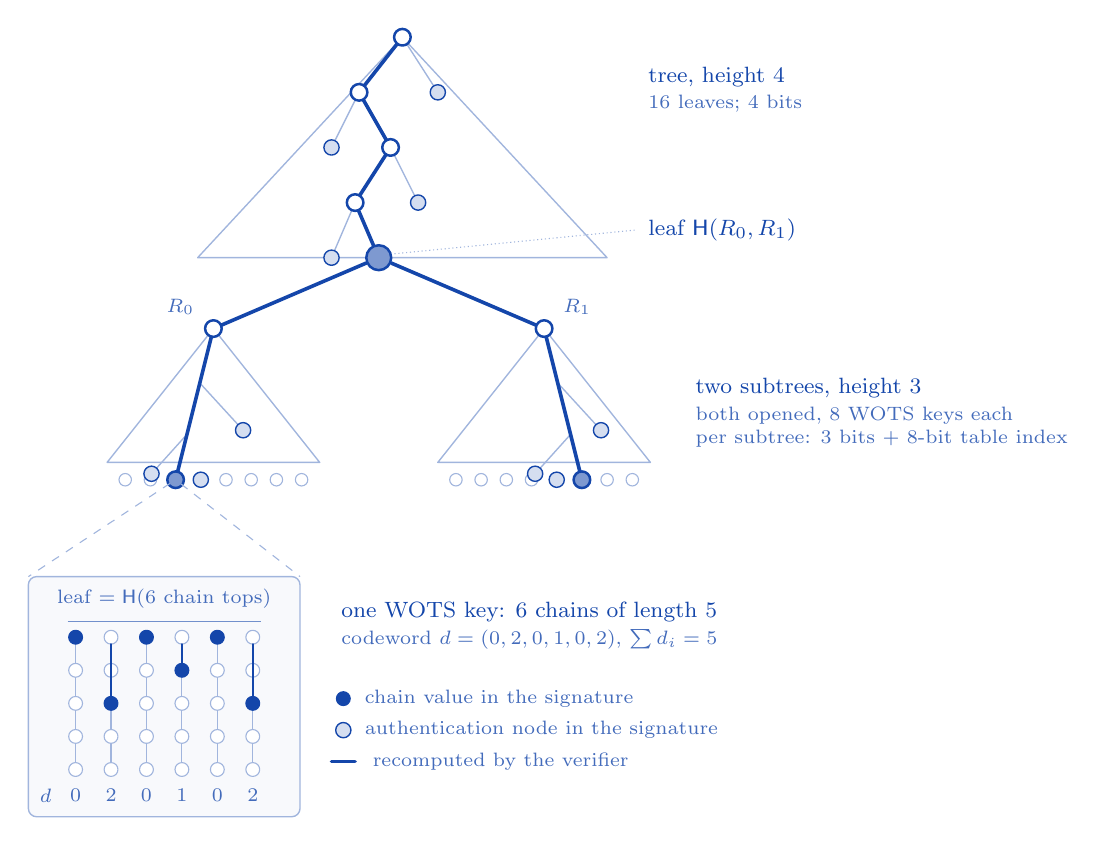
\begin{tikzpicture}[x=1cm,y=1cm,line join=round,
  tree/.style={draw=newfts!40,line width=0.5pt},
  path/.style={draw=newfts,line width=1.3pt,line cap=round},
  on/.style={circle,draw=newfts,line width=0.9pt,fill=white,minimum size=6pt,inner sep=0pt},
  auth/.style={circle,draw=newfts,line width=0.5pt,fill=newfts!18,minimum size=5.5pt,inner sep=0pt},
  off/.style={circle,draw=newfts!40,line width=0.4pt,fill=white,minimum size=4.5pt,inner sep=0pt},
  rev/.style={circle,draw=newfts,fill=newfts,minimum size=5pt,inner sep=0pt},
  hid/.style={circle,draw=newfts!40,line width=0.4pt,fill=white,minimum size=5pt,inner sep=0pt},
  lab/.style={font=\footnotesize,text=newfts},
  note/.style={font=\scriptsize,text=newfts!80}]
% ---------- top tree, height 4
\draw[tree] (0,6.4) -- (-2.6,3.6) -- (2.6,3.6) -- cycle;
\coordinate (t0) at (0,6.4);   \coordinate (t1) at (-0.55,5.7);
\coordinate (t2) at (-0.15,5.0); \coordinate (t3) at (-0.6,4.3); \coordinate (t4) at (-0.3,3.6);
\foreach \i/\j/\dx in {0/1/1.0,1/2/-0.75,2/3/0.8,3/4/-0.6} {
  \draw[tree] (t\i) -- ($(t\j)+(\dx,0)$);
  \node[auth] at ($(t\j)+(\dx,0)$) {};}
\draw[path] (t0) -- (t1) -- (t2) -- (t3) -- (t4);
\foreach \i in {0,...,3} \node[on] at (t\i) {};
\node[on,minimum size=9pt,fill=newfts!55] (sc) at (t4) {};
% ---------- two subtrees, height 3
\foreach \k/\cx/\pk in {0/-2.4/2,1/1.8/5} {
  \coordinate (r\k) at (\cx,2.7);
  \draw[tree] (r\k) -- (\cx-1.35,1.0) -- (\cx+1.35,1.0) -- cycle;
  \foreach \i in {0,...,7} \node[off] (c\k\i) at (\cx-1.12+0.32*\i,0.78) {};
  \coordinate (u3) at (c\k\pk);
  \coordinate (u1) at ($(r\k)!0.36!(u3)$); \coordinate (u2) at ($(r\k)!0.7!(u3)$);
  \draw[tree] (u1) -- ++(0.55,-0.6); \node[auth] at ($(u1)+(0.55,-0.6)$) {};
  \draw[tree] (u2) -- ++(-0.45,-0.5); \node[auth] at ($(u2)+(-0.45,-0.5)$) {};
  \node[auth] at ($(u3)+(\ifnum\pk>3 -0.32\else 0.32\fi,0)$) {};
  \draw[path] (sc) -- (r\k) -- (u3);
  \node[on] at (r\k) {};
  \node[on,fill=newfts!55] at (u3) {};
}
\node[note,anchor=south east] at ($(r0)+(-0.12,0.05)$) {$R_0$};
\node[note,anchor=south west] at ($(r1)+(0.12,0.05)$) {$R_1$};
% ---------- zoom on one WOTS key
\coordinate (B) at (-4.15,-2.9);   % lower-left chain node
\draw[newfts!40,line width=0.4pt,dashed] (c02) -- ($(B)+(-0.6,2.45)$);
\draw[newfts!40,line width=0.4pt,dashed] (c02) -- ($(B)+(2.85,2.45)$);
\draw[newfts!40,line width=0.5pt,rounded corners=3pt,fill=newfts!3] ($(B)+(-0.6,-0.6)$) rectangle ($(B)+(2.85,2.45)$);
\foreach \i/\d in {1/0,2/2,3/0,4/1,5/0,6/2} {
  \pgfmathsetmacro{\xx}{0.45*(\i-1)}
  \pgfmathtruncatemacro{\rv}{4-\d}
  \foreach \j in {0,...,3} \draw[newfts!40,line width=0.4pt] ($(B)+(\xx,0.42*\j)$) -- ($(B)+(\xx,0.42*\j+0.42)$);
  \foreach \j in {0,...,4} {\ifnum\j=\rv \node[rev] at ($(B)+(\xx,0.42*\j)$) {};
      \else \node[hid] at ($(B)+(\xx,0.42*\j)$) {}; \fi}
  \ifnum\rv<4 \draw[path,line width=0.9pt] ($(B)+(\xx,0.42*\rv+0.09)$) -- ($(B)+(\xx,1.59)$); \fi
  \node[note] at ($(B)+(\xx,-0.33)$) {$\d$};
}
\node[note] at ($(B)+(-0.38,-0.33)$) {$d$};
\draw[newfts!60,line width=0.4pt] ($(B)+(-0.1,1.88)$) -- ($(B)+(2.35,1.88)$);
\node[note,anchor=south] at ($(B)+(1.125,1.92)$) {leaf $=\hash(\text{6 chain tops})$};
% ---------- labels (right column)
\node[lab,anchor=west] at (3.0,5.9)  {tree, height 4};
\node[note,anchor=west] at (3.0,5.55) {16 leaves; 4 bits};
\node[lab,anchor=west] at (3.0,3.95) {leaf $\hash(R_0,R_1)$};
\draw[newfts!40,line width=0.4pt,densely dotted] (2.95,3.95) -- ($(sc)+(0.2,0.05)$);
\node[lab,anchor=west] at (3.6,1.95) {two subtrees, height 3};
\node[note,anchor=west] at (3.6,1.6) {both opened, 8 WOTS keys each};
\node[note,anchor=west] at (3.6,1.3) {per subtree: 3 bits $+$ 8-bit table index};
\node[lab,anchor=west] at (-0.9,-0.9) {one WOTS key: 6 chains of length 5};
\node[note,anchor=west] at (-0.9,-1.25) {codeword $d=(0,2,0,1,0,2)$, $\textstyle\sum d_i=5$};
% ---------- legend
\node[rev] at (-0.75,-2.0) {}; \node[note,anchor=west] at (-0.6,-2.0) {chain value in the signature};
\node[auth] at (-0.75,-2.4) {}; \node[note,anchor=west] at (-0.6,-2.4) {authentication node in the signature};
\draw[path] (-0.9,-2.8) -- (-0.6,-2.8); \node[note,anchor=west] at (-0.5,-2.8) {recomputed by the verifier};
\end{tikzpicture}

\small One of the 8 trees.
\end{center}

\paragraph{Encoding.} Bit fields and one 256-entry table: the encoding rejects no digest. Each tree takes 26 bits:
4 for the leaf, then, per subtree, 3 for the WOTS key and 8 for a table index. The 16 table indices are the first
16 bytes of the digest; its last 16 bytes, as a little-endian integer, hold the 16 WOTS keys, then the 8 leaves,
then the instance index, so no field lies across two 64-bit words. The table has 256 entries: sort the 246
codewords by decreasing $\sum_i d_i^2$, then in increasing lexicographic order (first digit most significant); entry $t$ is codeword number $t \bmod 214$.
Spread-out codewords are easier to forge once a key has signed twice, so the 32 most spread-out ones are left out,
and the 42 most concentrated ones appear twice. With the 24 bits of the instance index, the digest is 232 bits,
so it still takes one hash.

\paragraph{Costs.} Per tree:
\begin{itemize}
  \item size: 22 values, i.e.\ 6 chain values and 3 nodes per subtree, plus 4 nodes in the tree
  \item verification: 20 permutations, i.e.\ per subtree 5 chain steps, 1 for the leaf and 2 for the path, then 1 for
        $\hash(R_0,R_1)$ and 3 for the path in the tree
  \item signing: $16\cdot2\cdot8 = 256$ WOTS keys of 28 permutations each
\end{itemize}
Every signature has the same size and verification cost, and keygen is unchanged. The WOTS$^+$C key that signs
the forest uses a target sum of 123 instead of the 120 that would suit FORS: 3 fewer chain steps at verification,
for about 2\,200 counter tries instead of 830 when signing ($1.4\cdot10^3$ more permutations, still within the
signing costs of \cref{sec:scheme}).

\paragraph{Security.} A forgery at an instance with $r$ prior signatures needs every tree to be covered: in
both subtrees, the target WOTS key must have been opened, and the target codeword must lie below the componentwise
max of those openings. Let $f_t$ be the probability that $t$ random signatures by one WOTS key cover a random codeword
($f_1=0.0052$, $f_2=0.068$, $f_3=0.17$). Then
\[
\mathrm{cover}(r)=\Big(\sum_{u\ge1}\mathrm{Bin}(r,\tfrac1{16})(u)\Big[\sum_{t\ge1}\mathrm{Bin}(u,\tfrac18)(t)\,f_t\Big]^2\Big)^8 .
\]
The lifetime is the largest $N$ with $2^{127}\,2^{b-24}\,\mathbb{E}_{r\sim\mathrm{Poisson}(N/2^b)}[\mathrm{cover}(r)]\le1$:
the signatures spread over the $2^b$ instances of the kept subtree, and a forger's digest must also land in it.
The factor $2^{b-24}$ is what hypertree pruning~\cite{conduition} does not charge the forger: its rule reduces
the lifetime by the full pruning factor $2^{24-b}$, which is the signer's grinding cost, but the forger pays that
same cost per attempt. Here the credit is worth $2^{(24-b)/18}$, from $+14\%$ at $b=20$ to a factor 2 at $b=8$.
The same cover rule applied to FORS gives the first row, and the two-level forest is about 19\%
ahead at every subtree height. The best known attack also uses the WOTS$^+$C key (a counter search for a neighbouring
encoding, then one chain preimage): for both schemes it is up to 8\% below the cover figure at small $b$~\cite{proofs}. Every figure is rounded down. The last row holds the lifetimes proved in Lean~\cite{proofs}: an adversary
making $q$ hash queries forges with probability at most $q\cdot2^{-127}$.
\begin{center}
\setlength{\tabcolsep}{4.5pt}
\begin{tabular}{lrrrrrrr}
  \toprule
  $b$ & 24 & 20 & 14 & 13 & 12 & 10 & 8 \\
  \midrule
  FORS, cover & $3.00\cdot10^8$ & $2.20\cdot10^7$ & $4.33\cdot10^5$ & $2.24\cdot10^5$ & $1.16\cdot10^5$ & $3.14\cdot10^4$ & $8.4\cdot10^3$ \\
  forest, cover & $3.59\cdot10^8$ & $2.63\cdot10^7$ & $5.18\cdot10^5$ & $2.68\cdot10^5$ & $1.39\cdot10^5$ & $3.74\cdot10^4$ & $1.00\cdot10^4$ \\
  \midrule
  forest, proved & $3.36\cdot10^8$ & $2.38\cdot10^7$ & $4.41\cdot10^5$ & $2.26\cdot10^5$ & $1.16\cdot10^5$ & $3.08\cdot10^4$ & $8.1\cdot10^3$ \\
  \bottomrule
\end{tabular}
\end{center}

\begin{thebibliography}{99}
\bibitem{SP800230} Q.~Dang, D.~Moody. \emph{Additional SLH-DSA Parameter Sets for Limited-Signature Use
  Cases}. NIST SP~800-230 (draft), 2026. \url{https://csrc.nist.gov/pubs/sp/800/230/ipd}.
\bibitem{HK22C} A.~H\"ulsing, M.~Kudinov, E.~Ronen, E.~Yogev. \emph{SPHINCS$^+$C: Compressing SPHINCS$^+$
  With (Almost) No Cost}. IEEE S\&P, 2023. \url{https://eprint.iacr.org/2022/778}.
\bibitem{FIPS205} National Institute of Standards and Technology. \emph{Stateless Hash-Based Digital Signature
  Standard}. FIPS~205, 2024. \url{https://doi.org/10.6028/NIST.FIPS.205}.
\bibitem{proofs} \emph{leanSphincs proofs in Lean 4} (\texttt{LeanSphincs}, and \texttt{LeanForest} for
  \cref{sec:twolevel}), \texttt{formal/sphincs} in
  \url{https://github.com/TomWambsgans/leanXMSS-leanSPHINCS-candidates}.

\bibitem{hwbench} T.~Wambsgans. \emph{Hardware wallet benchmark}.
  \url{https://github.com/TomWambsgans/hardware-wallet-benchmark}.
\bibitem{conduition} conduition. \emph{Pruning Hypertrees for the Lax and Lazy}, 2026.
  \url{https://conduition.io/cryptography/hypertree-pruning/}.
\bibitem{CDI05} R.~Cramer, I.~Damg{\aa}rd, Y.~Ishai. \emph{Share Conversion, Pseudorandom Secret-Sharing and
  Applications to Secure Computation}. TCC, 2005. \url{https://doi.org/10.1007/978-3-540-30576-7_19}.
\bibitem{GS20} V.~Goyal, Y.~Song. \emph{Malicious Security Comes Free in Honest-Majority MPC}. CRYPTO, 2020.
  \url{https://eprint.iacr.org/2020/134}.
\bibitem{BGIN19} E.~Boyle, N.~Gilboa, Y.~Ishai, A.~Nof. \emph{Practical Fully Secure Three-Party
  Computation via Sublinear Distributed Zero-Knowledge Proofs}. ACM CCS, 2019.
  \url{https://eprint.iacr.org/2019/1390}.
\bibitem{PRAWNS} D.~Boneh, B.~B\"unz, J.~D., Y.~Litchev, K.~Nazirkhanova. \emph{PRAWNS: Threshold Hash-Based
  Signatures from Threshold PRFs}, 2026. \url{https://eprint.iacr.org/2026/2142}.
\bibitem{siggolf} J.~Nick (Blockstream). \emph{WCT-9: a WOTS-child forest replaces BPORS}, sig.golf
  submission, 2026. \url{https://github.com/Layr-Labs/sig.golf/commit/3321b777a511a6b454aad7ab721e8ab1af21c4d0}.
\end{thebibliography}

\end{document}
